\chapter{Результаты и заключение}

\section{Механизмы сосуществования в пространствах различных рамерностей}

В рамках нашего исследования предложено исследовать равновесные положения популяции в пространстве параметров модели, описанном выше, с ограничениями на некоторое подмножество параметров, которые приводит к нетривиальным стационарным точкам системы; такие ограничения также известны как \textit{механизмы сосуществования}, поскольку отсутствие нулевых стационарных решений есть выживание всех видов популяции.

\subsection{Competition-colonization trade-off}

В данной части работы мы приведем более точные иллюстрации для наблюдаемой реализации широко известного механизма \textbf{competition-colonization trade-off}; биологическое соображение, описывающее данный механизм, заключается в том, что сосуществование двух видов возможно, если один из видов сильнее конкурирует, а второй распространяется на большие расстояния, что в нашем пространстве можно наблюдать в пространстве $ \left[\sigma_{m2};\;d'_{12}\right] $ . Несложно заметить, что данное соображение описывает равновесные устойчивые положения модели «хищник–жертва».

Главной целью нашего исследования являются эффекты увеличения размерности геометрического пространства, в котором обитают особи. Рисунки [fig:cctod1], [fig:cctod2] and [fig:cctod3] иллюстрируют случаи $ \mathbb{R}^{1} $, $ \mathbb{R}^{2} $ и $ \mathbb{R}^{3} $ соответственно. В рамках выполнения работы нами был разработан численный метод, позволяющий считать решения системы точнее, чем ранее известные методы за счет экспоненциальной скорости сходимости и уменьшения выполняемых арифметических операций, что не позволяет ошибке накапливаться. Для каждого случая приведены два графика: поверхности плотностей индивидов (первых моментов) для каждой пары параметров $ (\sigma_{2}^{m};d'_{12}) $ и области в пространстве параметров, которые индуцируют сосуществование или существование только одного из видов (номер выживающего вида подписан на рисунке).

Исходя из полученных результатов, необходимо сделать следующий набор выводов и подчернуть следующие особенности:

\begin{itemize}
	\item интервал, выбранный для $ d'_{12} $ должен быть увеличен для получения более значимой области доминации более сильного вида; 
	
	\item общая идея мезанизма competition-colonization trade-off наблюдается во всех трех размерностях; при этом механизм нельзя воспринимать, как правило, необходимо требующее для сосуществования двух видов овердисперсии второго; как показано на наших рисунках, увеличение $ \sigma_{2}^{m} $ ведет к вымиранию сильного вида; 
	
	\item с ростом размерности геометрического пространства вид-колонизатор вытесняет более сильный вид и даже приводит к его вымиранию: общий тренд заключается в увеличении области выживания исключительно первого вида, в то время как область сосуществования двигается (двумерный случай) и уменьшается (трехмерный случай); 
	
	\item в трехмерном случае вид-колонизатор фактически приводит к вымиранию более сильного вида при всех рассмотренных наборах параметров модели; выделенная область сосуществования, несмотря на то, что оба вида там выживают, приводит к фактическому вымиранию более сильного вида, с резким ростом к границе области, где сильный вид выигрывает;
	
	\item как видно из рисунков [fig:cctod2:sub2] и [fig:cctod3:sub2] разработанный численный метод имеет несколько численных артефактов, которые можно устранить увеличением вычислительной точности нашего метода.
\end{itemize}

\begin{figure*}
	\centering
	\begin{subfigure}{.5\textwidth}
		\centering
		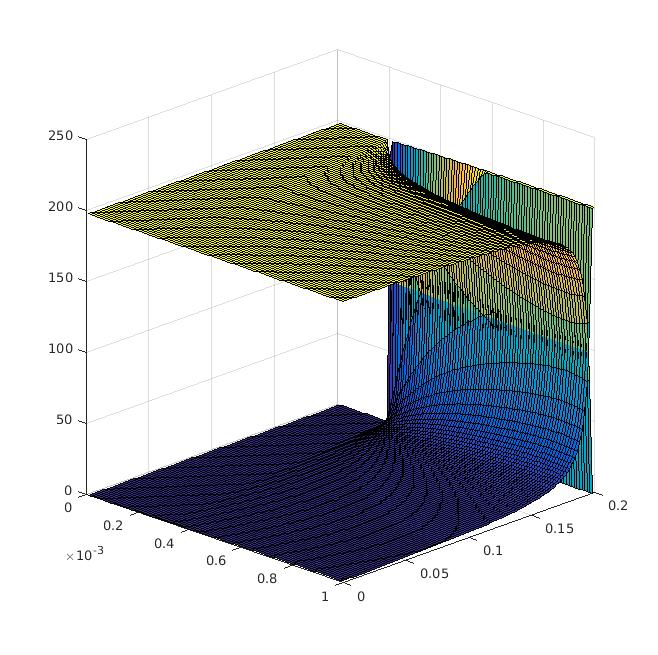
\includegraphics[width=.95\linewidth]{N1N2cctoD1.jpg}
		\caption{Surfaces of first moment \(N_1\) and \(N_2\) in described parameter space}
		\label{fig:cctod1:sub1}
	\end{subfigure}%
	\begin{subfigure}{.5\textwidth}
		\centering
		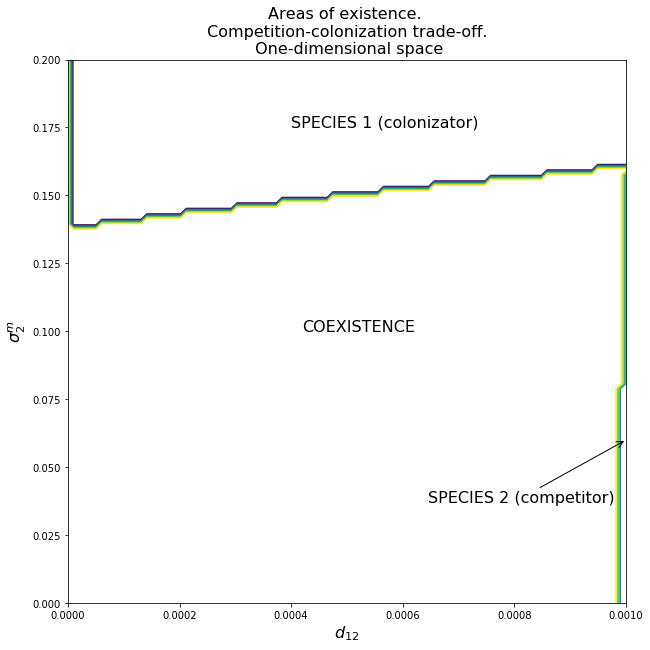
\includegraphics[width=.95\linewidth]{arccto08d1.png}
		\caption{Areas of coexistence in described parameter space} 
		\label{fig:cctod1:sub2}
	\end{subfigure}
		\begin{subfigure}{.5\textwidth}
		\centering
		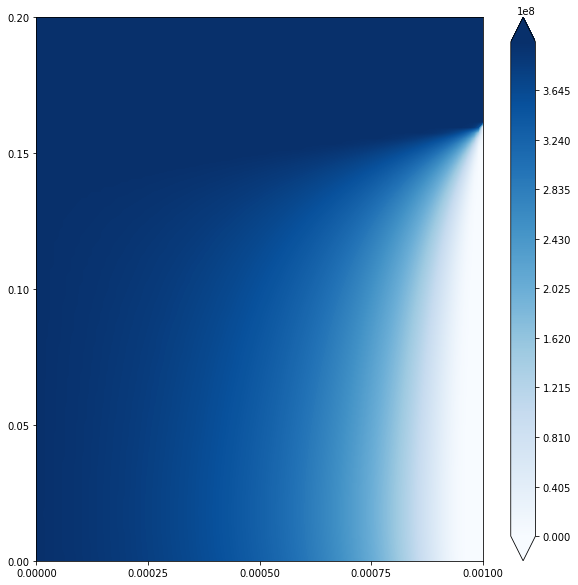
\includegraphics[width=.95\linewidth]{ccto_d1_n1.png}
		\caption{Surfaces of first moment \(N_1\) and \(N_2\) in described parameter space}
		\label{fig:cctod1:sub3}
	\end{subfigure}%
	\begin{subfigure}{.5\textwidth}
		\centering
		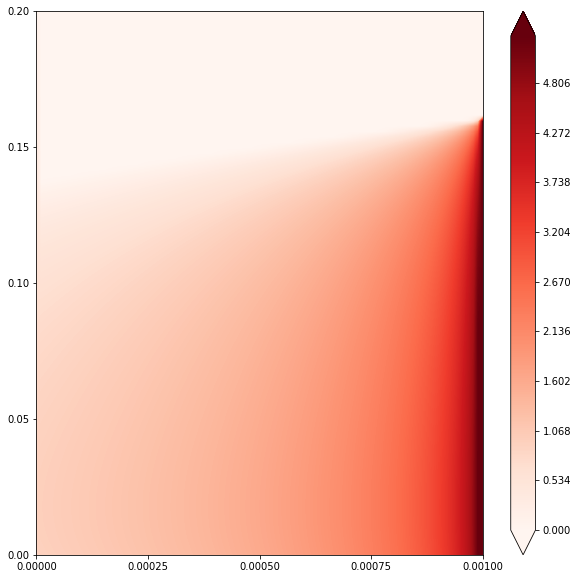
\includegraphics[width=.95\linewidth]{ccto_d1_n2.png}
		\caption{Areas of coexistence in described parameter space} 
		\label{fig:cctod1:sub4}
	\end{subfigure}
	\caption{Realization of Competition-Colonization Trade-Off mechanisms in $\sigma^m_2$ and $d'_{12}$ parameter space in case of \emph{one-dimensional habitat}. Other parameters are chosen as follows:  $b_{1}=b_{2}=0.4
		, d_{1}=d_{2}=0.2
		, d'_{11}=d'_{22}=d'_{21}=0.001,
		\sigma_{1}^{m}=0.04
		, \sigma_{11}^{w}=\sigma_{12}^{w}=\sigma_{21}^{w}=\sigma_{22}^{w}=0.04$}
	\label{fig:cctod1}
\end{figure*}

\begin{figure*}
	\centering
	\begin{subfigure}{.5\textwidth}
		\centering
		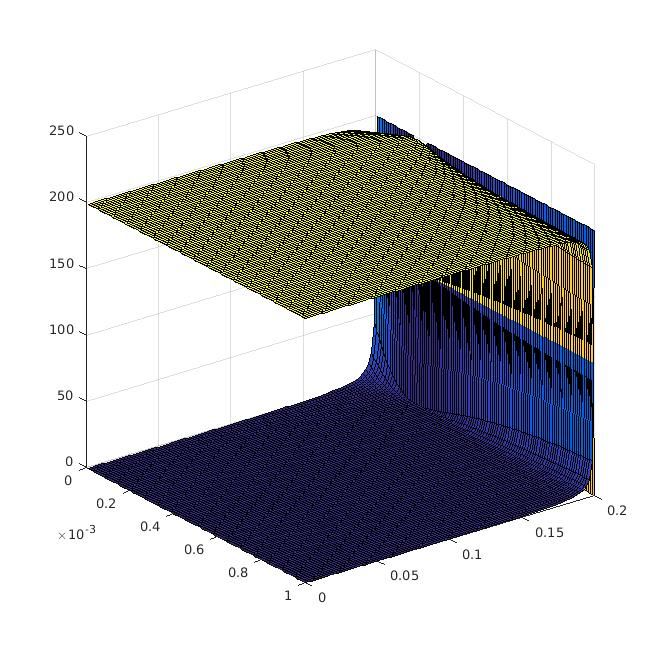
\includegraphics[width=.95\linewidth]{N1N2cctoD2.jpg}
		\caption{Surfaces of first moment \(N_1\) and \(N_2\) in described parameter space}
		\label{fig:cctod2:sub1}
	\end{subfigure}%
	\begin{subfigure}{.5\textwidth}
		\centering
		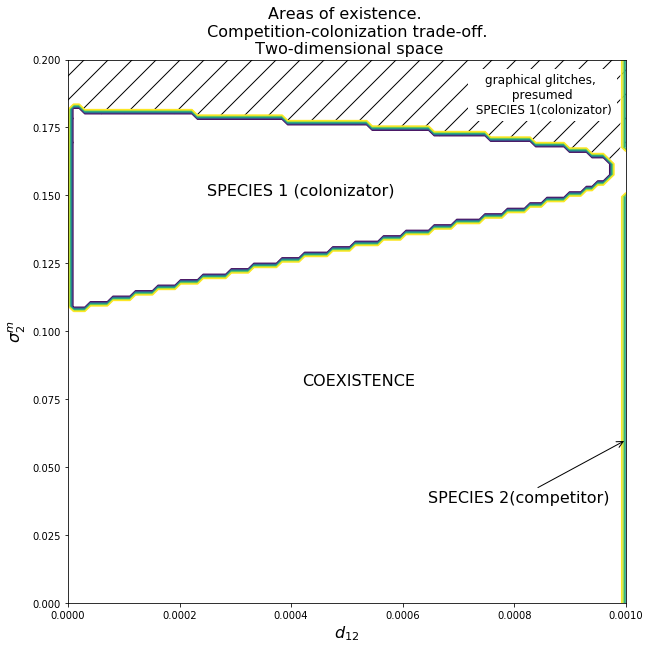
\includegraphics[width=.95\linewidth]{arccto08d2.png}
		\caption{Areas of coexistence in described parameter space}
		\label{fig:cctod2:sub2}
	\end{subfigure}
	\centering
	\begin{subfigure}{.5\textwidth}
		\centering
		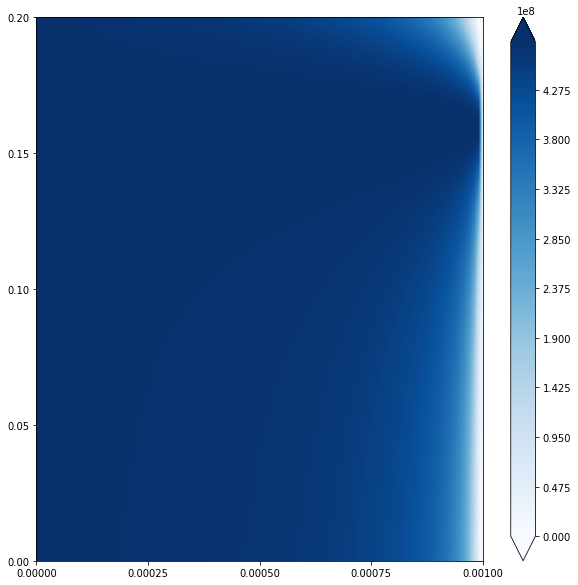
\includegraphics[width=.95\linewidth]{ccto_d2_n1.png}
		\caption{Surfaces of first moment \(N_1\) and \(N_2\) in described parameter space}
		\label{fig:cctod2:sub3}
	\end{subfigure}%
	\begin{subfigure}{.5\textwidth}
		\centering
		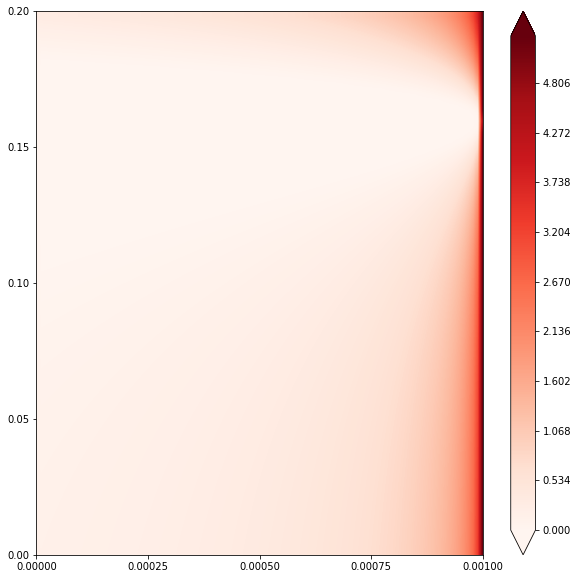
\includegraphics[width=.95\linewidth]{ccto_d2_n2.png}
		\caption{Areas of coexistence in described parameter space}
		\label{fig:cctod2:sub4}
	\end{subfigure}
	\caption{Realization of Competition-Colonization Trade-Off mechanims in $\sigma^m_2$ and $d'_{12}$ parameter space in case of \emph{two-dimensional habitat}. Other parameters are chosen as follows:  $b_{1}=b_{2}=0.4
		, d_{1}=d_{2}=0.2
		, d'_{11}=d'_{22}=d'_{21}=0.001,
		\sigma_{1}^{m}=0.04
		, \sigma_{11}^{w}=\sigma_{12}^{w}=\sigma_{21}^{w}=\sigma_{22}^{w}=0.04$}
	\label{fig:cctod2}
\end{figure*}


\begin{figure*}
	\centering
	\begin{subfigure}{.5\textwidth}
		\centering
		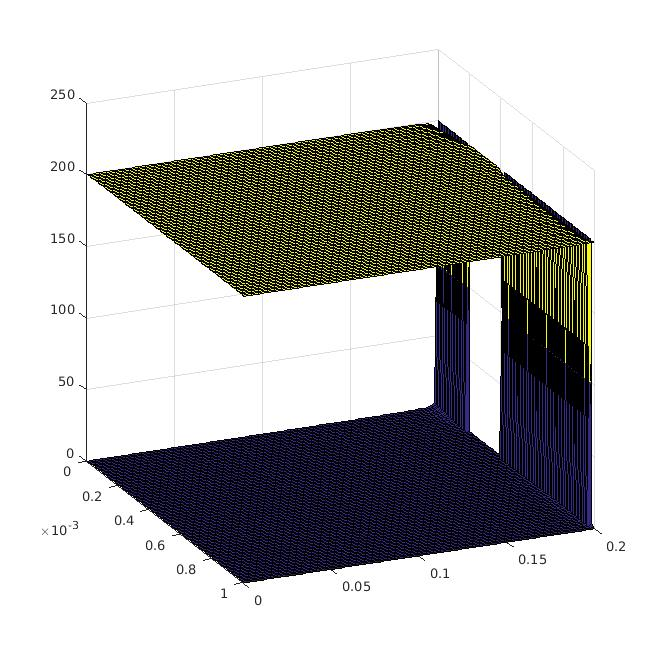
\includegraphics[width=.95\linewidth]{N1N2cctoD3.jpg}
		\caption{Surfaces of first moment \(N_1\) and \(N_2\) in described parameter space}
		\label{fig:cctod3:sub1}
	\end{subfigure}%
	\begin{subfigure}{.5\textwidth}
		\centering
		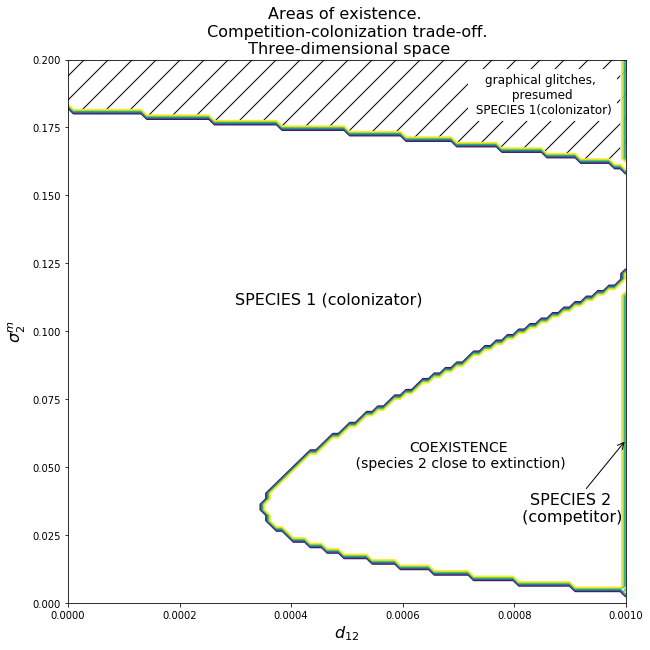
\includegraphics[width=.95\linewidth]{arccto08d3.png}
		\caption{Areas of coexistence in described parameter space}
		\label{fig:cctod3:sub2}
	\end{subfigure}
\centering
\begin{subfigure}{.5\textwidth}
	\centering
	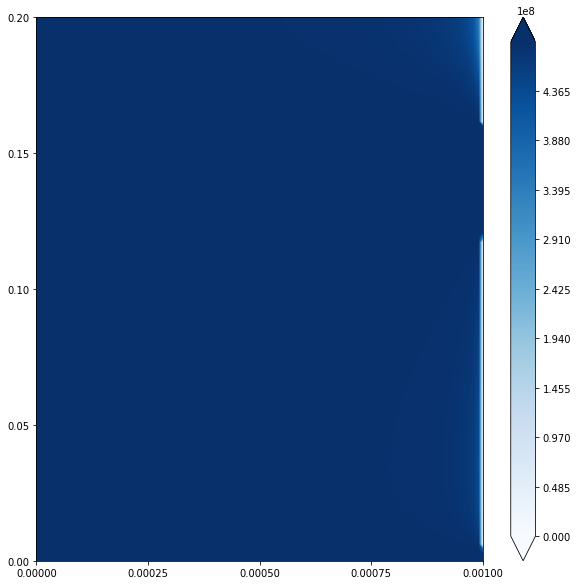
\includegraphics[width=.95\linewidth]{ccto_d3_n2.png}
	\caption{Surfaces of first moment \(N_1\) and \(N_2\) in described parameter space}
	\label{fig:cctod3:sub3}
\end{subfigure}%
\begin{subfigure}{.5\textwidth}
	\centering
	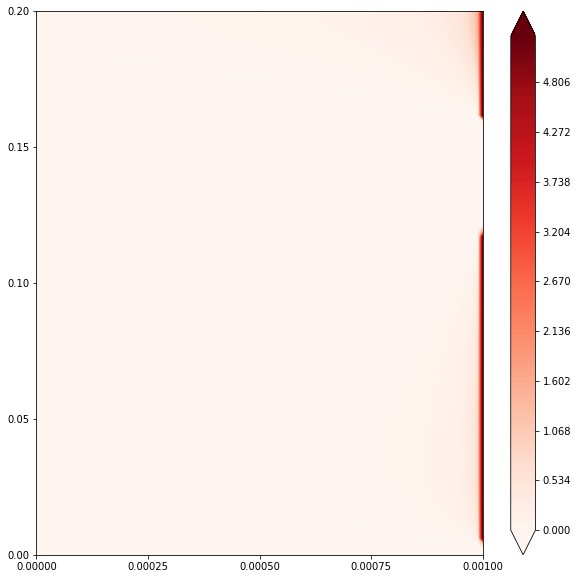
\includegraphics[width=.95\linewidth]{ccto_d3_n1.png}
	\caption{Areas of coexistence in described parameter space}
	\label{fig:cctod3:sub4}
\end{subfigure}
	\caption{Realization of Competition-Colonization Trade-Off mechanisms in $\sigma^m_2$ and $d'_{12}$ parameter space in case of \emph{three-dimensional habitat}. Other parameters are chosen as follows:  $b_{1}=b_{2}=0.4
		, d_{1}=d_{2}=0.2
		, d'_{11}=d'_{22}=d'_{21}=0.001,
		\sigma_{1}^{m}=0.04
		, \sigma_{11}^{w}=\sigma_{12}^{w}=\sigma_{21}^{w}=\sigma_{22}^{w}=0.04$}
	\label{fig:cctod3}
\end{figure*}



\subsection{Heteromyopia}

В данной части работы мы рассмотрим другой механизм сосуществования, который был предложен в [25], \textit{heteromyopia}: драйвером сосуществования в рамках данного механизма считается принцип о том, что межвидовая конкуренция индивидов проходит на меньшем расстоянии, чем внутривидовая. В нашей модели мы нашли данный механизм в пространстве параметров $ \left[\sigma_{ii}^{w};\sigma_{ij}^{w}\right] $.

Главной целью нашего исследования являются эффекты увеличения размерности геометрического пространства, в котором обитают особи. Рисунки [fig:cctod1], [fig:cctod2] and [fig:cctod3] иллюстрируют случаи $ \mathbb{R}^{1} $, $ \mathbb{R}^{2} $ и $ \mathbb{R}^{3} $ соответственно. В рамках выполнения работы нами был разработан численный метод, позволяющий считать решения системы точнее, чем ранее известные методы за счет экспоненциальной скорости сходимости и уменьшения выполняемых арифметических операций, что не позволяет ошибке накапливаться. Для каждого случая приведены два графика: поверхности плотностей индивидов (первых моментов) для каждой пары параметров $ \left[\sigma_{ii}^{w};\sigma_{ij}^{w}\right] $ и области в пространстве параметров, которые индуцируют сосуществование или существование только одного из видов (номер выживающего вида подписан на рисунке).

Исходя из полученных результатов, необходимо сделать следующий набор выводов и подчернуть следующие особенности:

\begin{itemize}
	\item в целом, корректность предложенного механизма была подтверждена в случае одномерного и двумерного пространства обитания; стоит также отметить, что предложенная в оригинальной статье линейность зависимости между радиусом интравидовой и интервидовой конкуренции является неплохим, но не самым лучшим первым приболижением; 
	
	\item описанный механизм отсутствует в случае двумерной среды обитания, что ставит вопросы о его значимости и корректности; 
	
	\item согласно рисункам [fig:hmd1:sub2], [fig:hmd2:sub2] и [fig:hmd3:sub2] разработанный численный метод, как и в случае рисунков для competition-colonization trade-off выше, содержит набор численных артефактов.
\end{itemize}

\begin{figure*}[ht]
	\centering
	\begin{subfigure}{.5\textwidth}
		\centering
		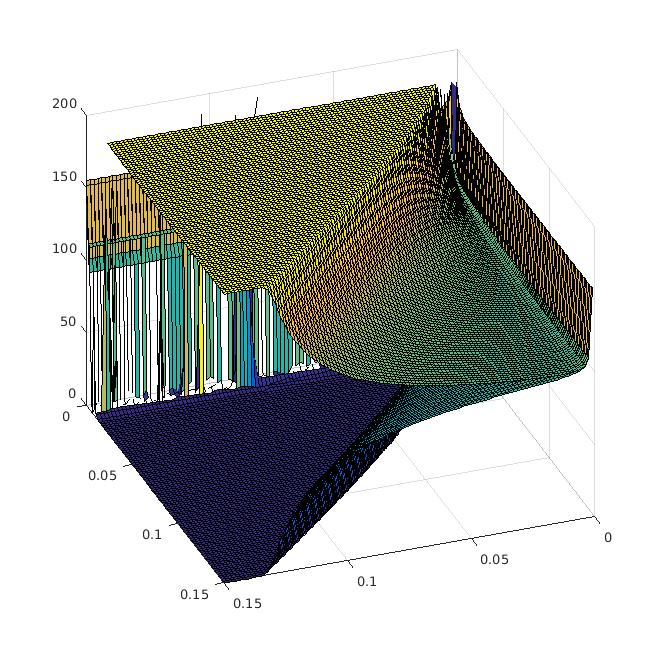
\includegraphics[width=.93\linewidth]{N1N2hm08D1.jpg}
		\caption{Surfaces of first moment \(N_1\) and \(N_2\) in described parameter space}
		\label{fig:hmd1:sub1}
	\end{subfigure}%
	\begin{subfigure}{.5\textwidth}
		\centering
		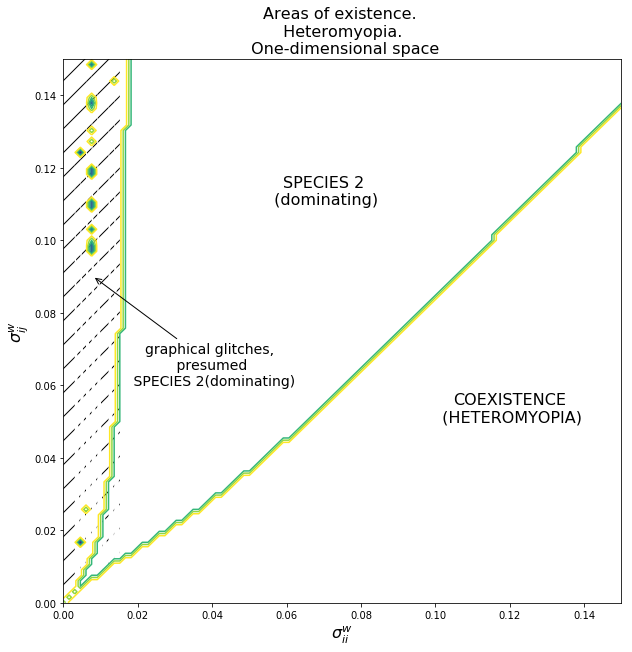
\includegraphics[width=.93\linewidth]{arhm08d1.png}
		\caption{Areas of coexistence in described parameter space} 
		\label{fig:hmd1:sub2}
	\end{subfigure}
\begin{subfigure}{.5\textwidth}
	\centering
	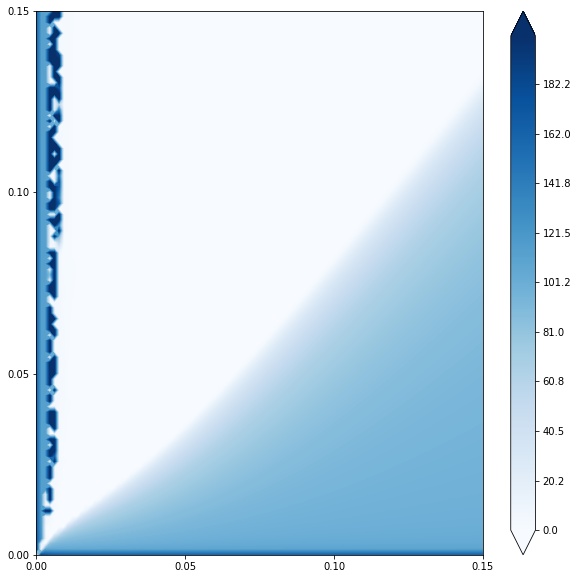
\includegraphics[width=.93\linewidth]{hm_d1_n1.png}
	\caption{Surfaces of first moment \(N_1\) and \(N_2\) in described parameter space}
	\label{fig:hmd1:sub3}
\end{subfigure}%
\begin{subfigure}{.5\textwidth}
	\centering
	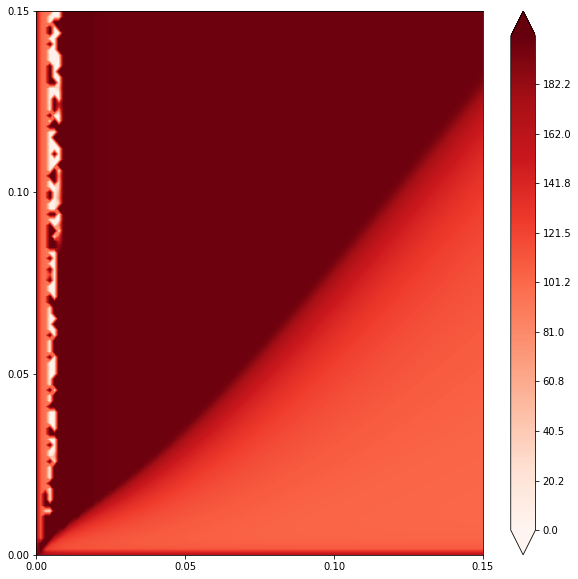
\includegraphics[width=.93\linewidth]{hm_d1_n2.png}
	\caption{Areas of coexistence in described parameter space} 
	\label{fig:hmd1:sub4}
\end{subfigure}
	\caption{Realization of Heteromyopia mechanisms in  $\sigma_{11}^{w}=\sigma_{22}^{w}$ and $\sigma_{12}^{w}=\sigma_{21}^{w}$ parameter space in case of \emph{one-dimensional habitat}. Other parameters are chosen as follows: $b_{1}=b_{2}=0.4
		, d_{1}=d_{2}=0.2
		, d'_{11}=d'_{22}=d'_{21}=d'_{12}=0.001,
		\sigma_{1}^{m}=\sigma_{2}^{m}=0.06$. }
	\label{fig:hmd1}
\end{figure*}

\begin{figure*}[ht]
	\centering
	\begin{subfigure}{.5\textwidth}
		\centering
		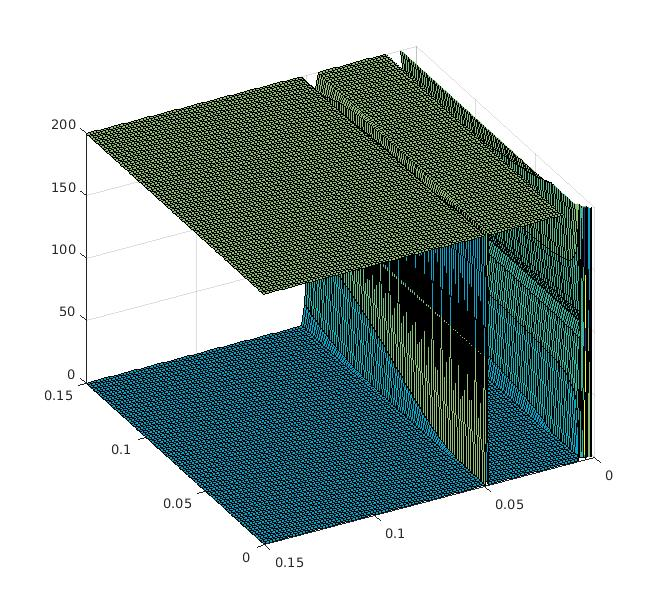
\includegraphics[width=.93\linewidth]{N1N2hm04D2.jpg}
		\caption{Surfaces of first moment \(N_1\) and \(N_2\) in described parameter space}
		\label{fig:hmd2:sub1}
	\end{subfigure}%
	\begin{subfigure}{.5\textwidth}
		\centering
		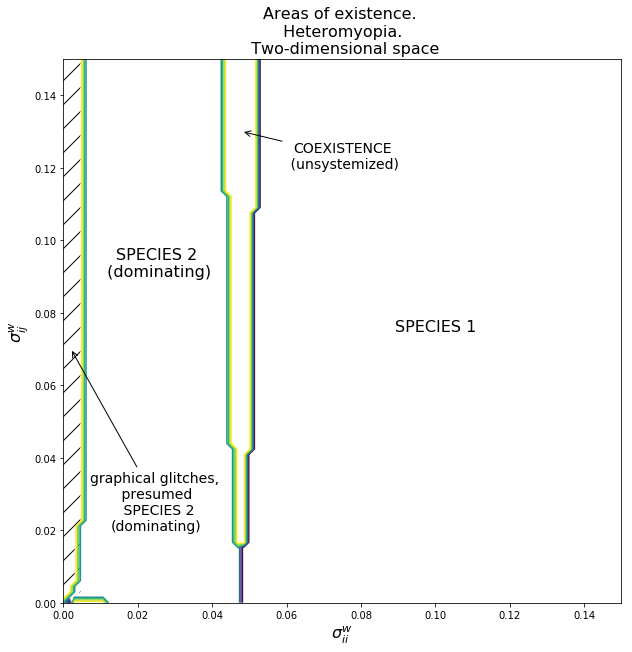
\includegraphics[width=.93\linewidth]{arhm08d2.png}
		\caption{Areas of coexistence in described parameter space}
		\label{fig:hmd2:sub2}
	\end{subfigure}
\begin{subfigure}{.5\textwidth}
	\centering
	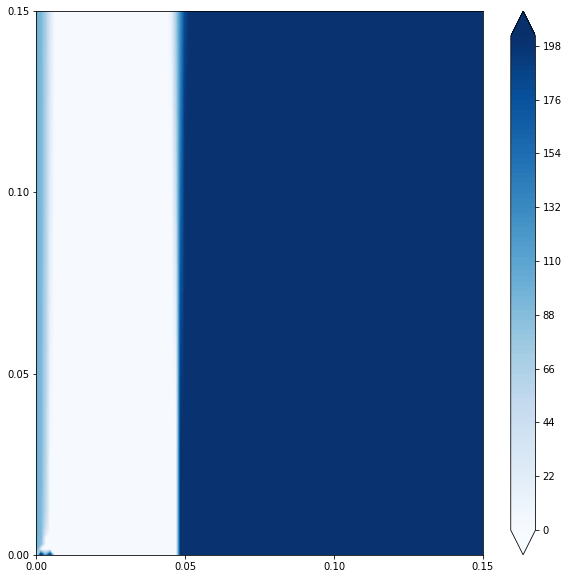
\includegraphics[width=.93\linewidth]{hm_d2_n1.png}
	\caption{Surfaces of first moment \(N_1\) and \(N_2\) in described parameter space}
	\label{fig:hmd2:sub3}
\end{subfigure}%
\begin{subfigure}{.5\textwidth}
	\centering
	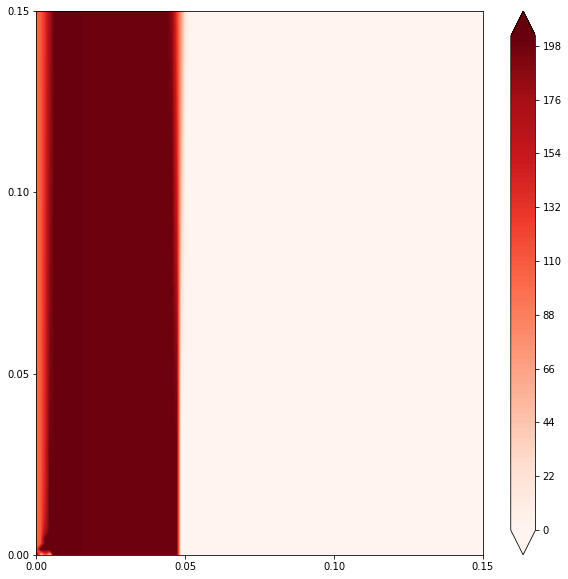
\includegraphics[width=.93\linewidth]{hm_d2_n2.png}
	\caption{Areas of coexistence in described parameter space}
	\label{fig:hmd2:sub4}
\end{subfigure}
	\caption{Realization of Heteromyopia mechanisms in  $\sigma_{11}^{w}=\sigma_{22}^{w}$ and $\sigma_{12}^{w}=\sigma_{21}^{w}$ parameter space in case of \emph{two-dimensional habitat}. Other parameters are chosen as follows: $b_{1}=b_{2}=0.4
		, d_{1}=d_{2}=0.2
		, d'_{11}=d'_{22}=d'_{21}=d'_{12}=0.001,
		\sigma_{1}^{m}=\sigma_{2}^{m}=0.06$. }
	\label{fig:hmd2}
\end{figure*}

\begin{figure*}[ht]
	\centering
	\begin{subfigure}{.5\textwidth}
		\centering
		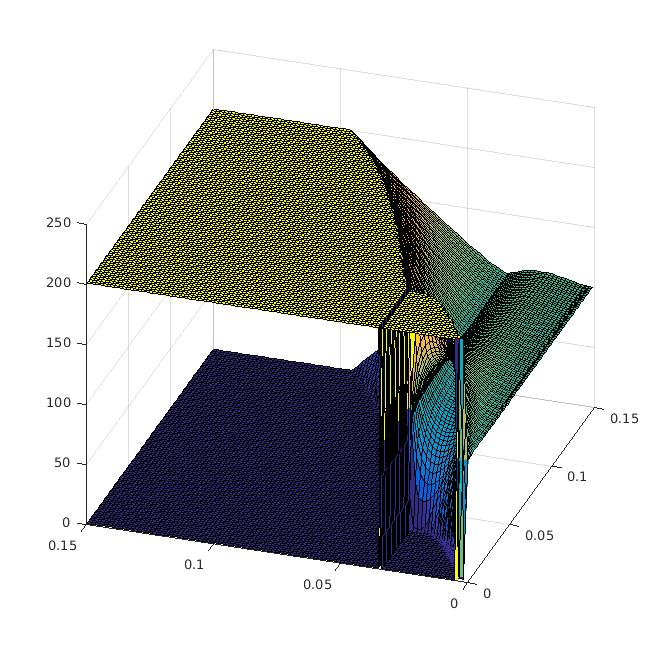
\includegraphics[width=.93\linewidth]{N1N2hm08D3.jpg}
		\caption{Surfaces of first moment \(N_1\) and \(N_2\) in described parameter space}
		\label{fig:hmd3:sub1}
	\end{subfigure}%
	\begin{subfigure}{.5\textwidth}
		\centering
		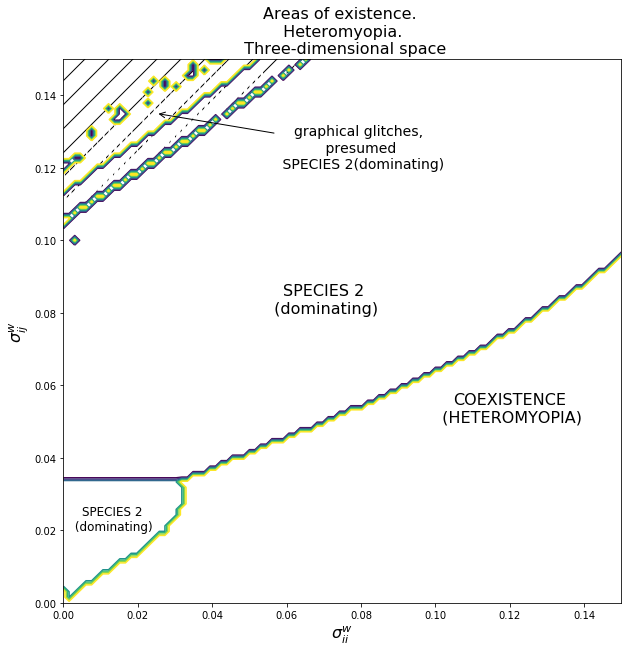
\includegraphics[width=.93\linewidth]{arhm08d3.png}
		\caption{Areas of coexistence in described parameter space}
		\label{fig:hmd3:sub2}
	\end{subfigure}
	\begin{subfigure}{.5\textwidth}
	\centering
	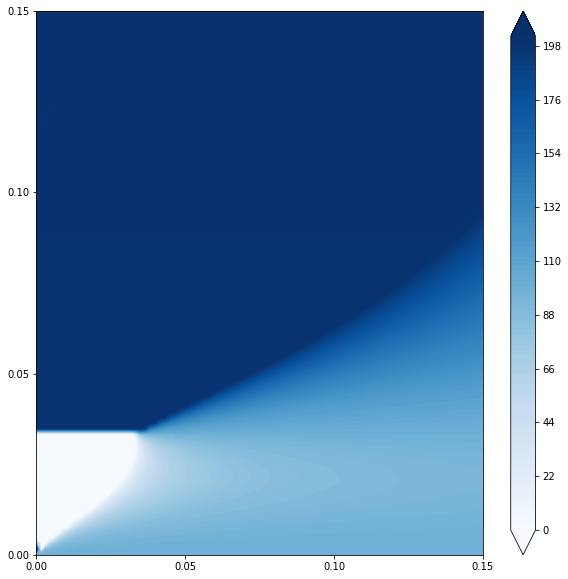
\includegraphics[width=.93\linewidth]{hm_d3_n1.png}
	\caption{Surfaces of first moment \(N_1\) and \(N_2\) in described parameter space}
	\label{fig:hmd3:sub3}
\end{subfigure}%
\begin{subfigure}{.5\textwidth}
	\centering
	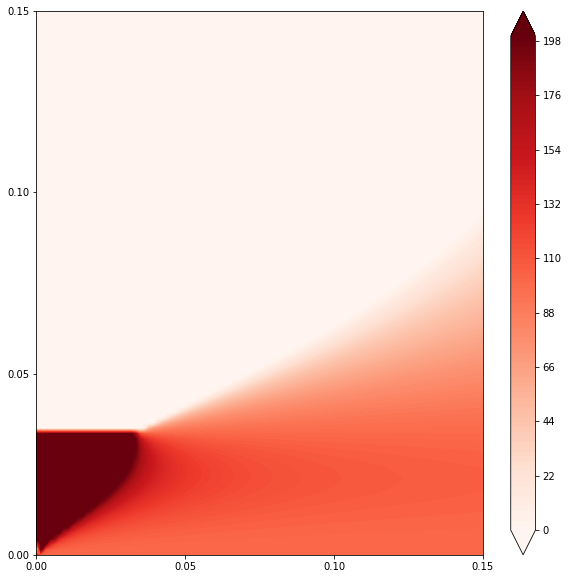
\includegraphics[width=.93\linewidth]{hm_d3_n2.png}
	\caption{Areas of coexistence in described parameter space}
	\label{fig:hmd3:sub4}
\end{subfigure}
	\caption{Realization of Heteromyopia mechanisms in  $\sigma_{11}^{w}=\sigma_{22}^{w}$ and $\sigma_{12}^{w}=\sigma_{21}^{w}$ parameter space in case of \emph{three-dimensional habitat}. Other parameters are chosen as follows: $b_{1}=b_{2}=0.4
		, d_{1}=d_{2}=0.2
		, d'_{11}=d'_{22}=d'_{21}=d'_{12}=0.001,
		\sigma_{1}^{m}=\sigma_{2}^{m}=0.06$. }
	\label{fig:hmd3}
\end{figure*}


\subsection{Дальнейшее исследование}

Помимо полученных выше выводов и указанных дальнейших шагов по их преодолению, хотелось бы отдельно указать еще несколько этапов и целей для дальнешей работы:

\begin{enumerate}
	
\item Проведение биологических симуляций (часть из них уже была сделана, результаты могут быть обнаружены в том же репозитории, что и головной код численного метода) для получения тестовой выборки, на которой можно будет проверить корректность аппроксимации третьего момента и улучшить ее;

\item  Изучение случае больших размерностей; несмотря на кажущуюся математичность и неприменимость подобных сред обитания в реальной жизни, необходимо отметить, что более чем трехмерные пространства — это классический подход моделирования биоценозов тропических лесов;

\item Изучение работы численного метода и зависимости результатов от ядер другого вида; в частности, рассмотрение ядер конкуренции с сингулярностью в 0, что позволяет моделировать размер индивида, и ядер дисперсии с 0 в 0, что является более корректным биологическим случаем;

\item Получение корректных ядер взаимодействия в модели, согласно имеющимся датасетам о распределении планктона в течениях; центральная сложность данной задачи заключается в том, что получение корректной выборочной фукнции распределения затруднена наличием градиентов течения и кислорода, влияние которых должно быть учтено при моделировании;

\item Изучение поведение симбионтов (т.е. видов в отрицательной константой конкуренции) с учетом пространственной структуры и наличием внутривидовой конкуренции.

\end{enumerate}